\documentclass{article}
\usepackage{bbm}
\usepackage{listings}
\usepackage{amsmath}
\usepackage[final]{pdfpages}
\usepackage{graphicx}

\title{Bayesian Statistics Homework1}

\author{
  Adam Li \\
  Department of Biomedical Engineering\\
  Johns Hopkins University\\
  Baltimore, MD 21210 \\
  \texttt{ali39@jhu.edu} \\
}

\begin{document}

\maketitle

\section{Problem 1}
$Y_1,Y_2,...,Y_6$ are observations from a uniform distribution ($\theta - 1/2, \theta + 1/2$) in order: 10.9, 11.0, 11.1, 11.4, 11.5, 11.7. The prior is uniform (10, 20).

$$P(\theta) \sim uniform(10,20)$$
$$L(Y|\theta) = \prod_{i=1}^6 \mathbbm{1}{(\theta - 1/2 < Y_i < \theta + 1/2)}$$

$L(Y|\theta)$ would just be an intersection of the indicator functions. For example, $\mathbbm{1}{(\theta - 1/2 < 10.9 < \theta + 1/2)} = \mathbbm{1}{(10.4 < \theta < 11.4)}$.


The indicator functions give the following constraints: \\
$\mathbbm{1}{(10.4 < \theta < 11.4)}$ \\
$\mathbbm{1}{(10.5 < \theta < 11.5)}$ \\
$\mathbbm{1}{(10.6 < \theta < 11.6)}$ \\
$\mathbbm{1}{(10.9 < \theta < 11.9)}$ \\
$\mathbbm{1}{(11.0 < \theta < 12.0)}$ \\
which gives $\mathbbm{1}{(11.0 < \theta < 11.4)}$ 

The posterior distribution is $P(\theta|Y) \propto L(\theta)P(\theta) = \mathbbm{1}{(11.0 < \theta < 11.4)} \frac{1}{10} \mathbbm{1}{(10.0 < \theta < 20.0)} = \mathbbm{1}{(11.0 < \theta < 11.4)} \frac{1}{10}$ 

The posterior distribution $P(\theta|Y) \sim uniform (11.0, 11.4)$

\section{Problem 2}
\subsection{i}
$P(x|y,z) = \frac{P(y,z|x)P(x)}{P(y,z)} = \frac{P(x,y,z)}{P(y,z)}$

$= \frac{P(x,y,z)}{\int\!{P(x,y,z)dx}} = \frac{f(x,z)g(y,z)h(z)}{\int\!{f(x,z)g(y,z)h(z)dx}} = \frac{f(x,z)}{\int\!{f(x,z)dx}}$

\subsection{ii}
$P(y|x,z) = \frac{P(x,z|y)P(y)}{P(x,z)} = \frac{P(x,y,z)}{P(x,z)}$

$= \frac{P(x,y,z)}{\int\!{P(x,y,z)dy}} = \frac{f(x,z)g(y,z)h(z)}{\int\!{f(x,z)g(y,z)h(z)dy}} = \frac{g(y,z)}{\int\!{g(y,z)dy}}$

\subsection{iii}
We want to show,
$P(x,y|z) = P(y|z)P(x|z)$

\section{Problem 3}
$$P(\theta) \sim gamma(x, k)$$
$$P(Y|\theta) \sim exp(\theta)$$


With $P(\theta) = constant * \theta^{k-1}e^{-\theta/x}$, with $E[\theta]=0.2=k\theta$ and $Var[\theta]=1=k\theta^2$, so it is gamma(5, 1/25) = gamma(x, k).


$L(\theta) = \prod_{i=1}^NP(Y_i|\theta) = \lambda^Ne^{-\lambda\sum_{i=1}^NY_i}$, and we know the average = 3.8, so $\sum{i=1}^NY_i = N*3.8$.


The posterior distribution is $P(\theta|Y) \propto L(\theta)P(\theta) = L(\theta)gamma(x,k) = \theta^{k+N-1}e^{-\theta(\sum Y_i + 1/x)} * constant$.


The posterior distribution is $\sim gamma(\frac{1}{\sum Y_i + 1/x}, k + N)$. where k is known, x is known and the sum of $Y_i$ are known. 

\section{Problem 4}
The negative binomial distribution is defined for an unknown theta and r. k is defined as the number of successes from all samples.

Consider $Y_1, ..., Y_N$ observations that = 1 if successful and 0 otherwise, where $\sum Y_i = k$

$$P(\theta) \sim beta(a,b)$$
$$L(Y|\theta) = \prod_{i=1}^N \theta^{\sum Y_i} (1-\theta)^r * constant$$

The posterior distribution is $P(\theta|Y) \propto P(\theta)L(Y|\theta) = \theta^{a-1}(1-\theta)^{b-1}(1-\theta)^{r}\theta^{\sum Y_i} * constant = \theta^{a+\sum Y_i - 1} (1-\theta)^{b+r-1}$. 

This is $\sim beta(a + \sum Y_i, b+r)$, which shows that the beta distribution is a conjugate family for the negative binomial distribution. 

\section{Problem 5}
\subsection{i}
This is just the joint distribution of many Bernoulli's, which is the Binomial distribution.

$P(Y_1=y_1,...,Y_{100}=y_{100}|\theta = {100 \choose k} \theta^k (1-\theta)^{100-k}$

The probability of the sum given theta, though does not look at the order of Bernoulli trials, but just at the sum. It is therefore

$P(\sum Y_i = y|\theta = \theta^k (1-\theta)^{100-k}$

\subsection{ii}
See R Code.

%----- Dimensions -----
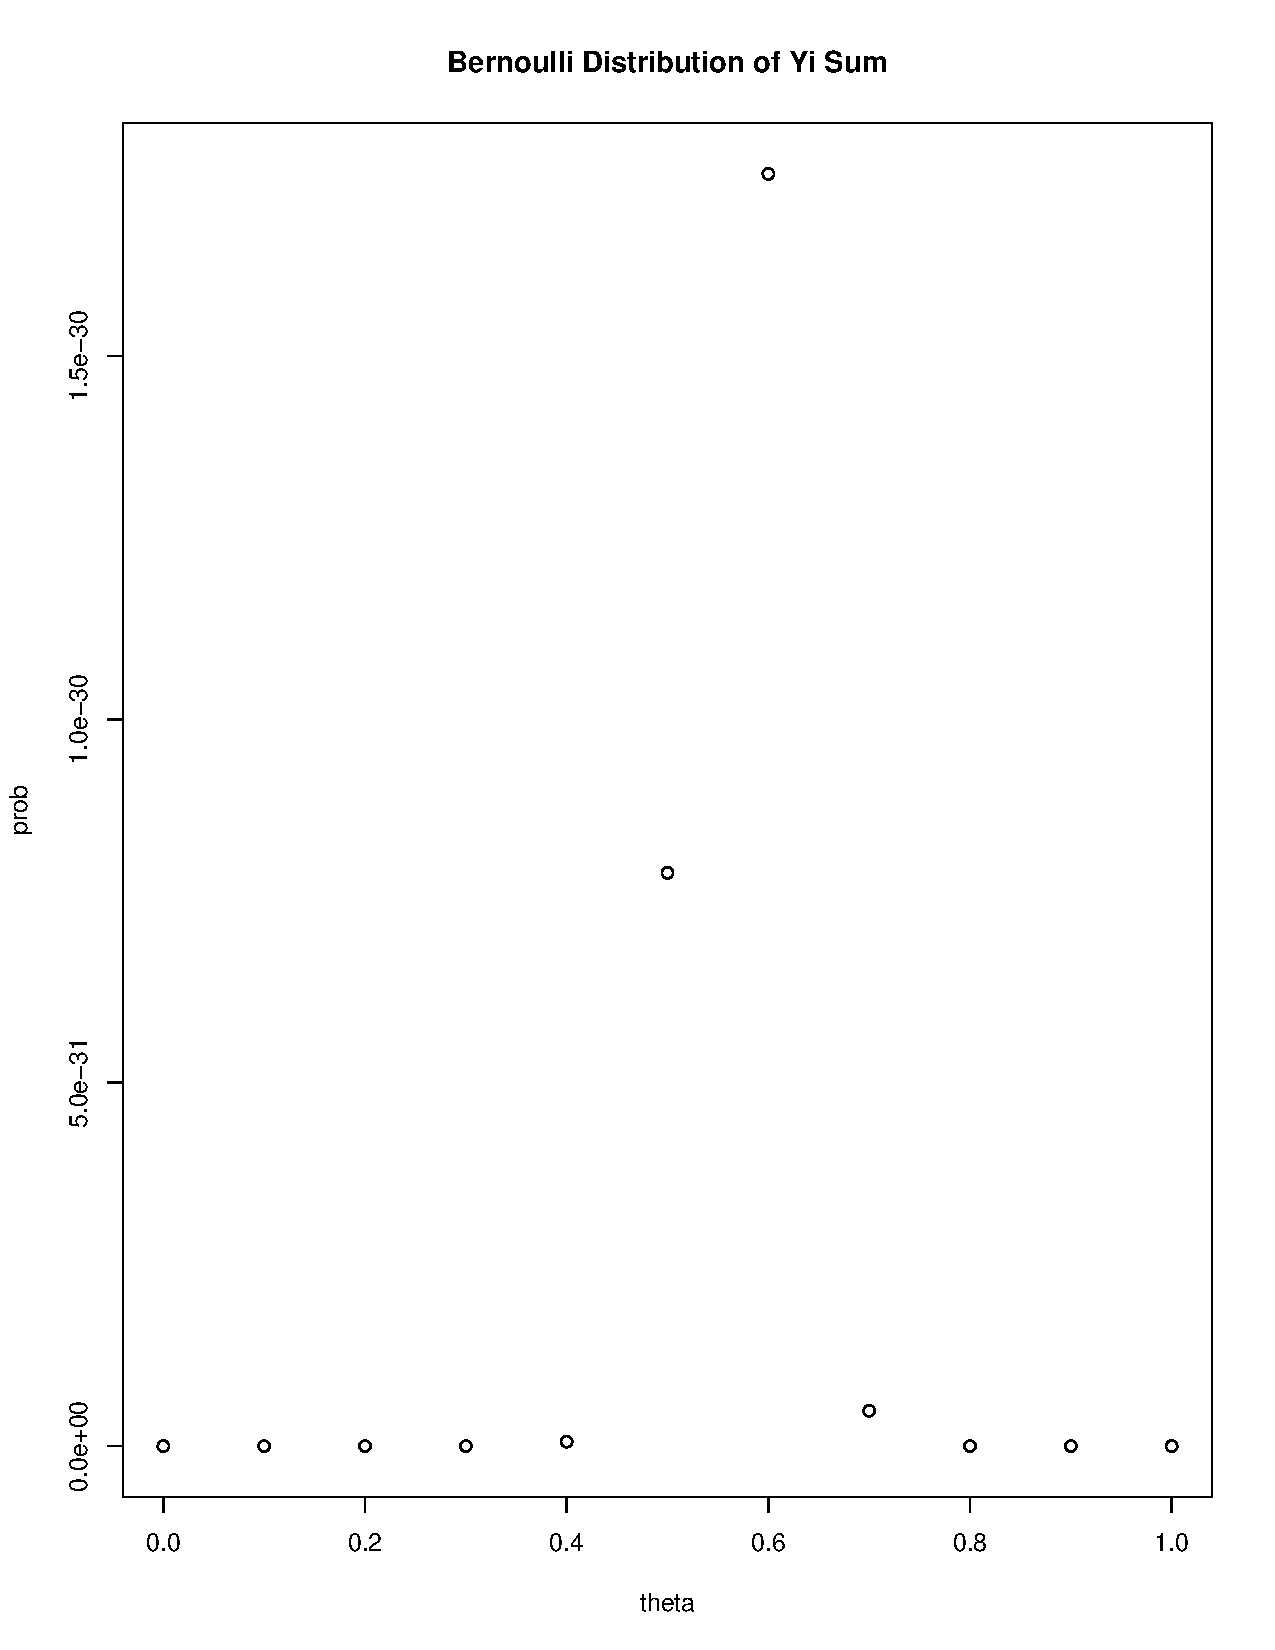
\includegraphics[width=75mm, scale=0.8]{5ii_plot.pdf}

\subsection{iii}
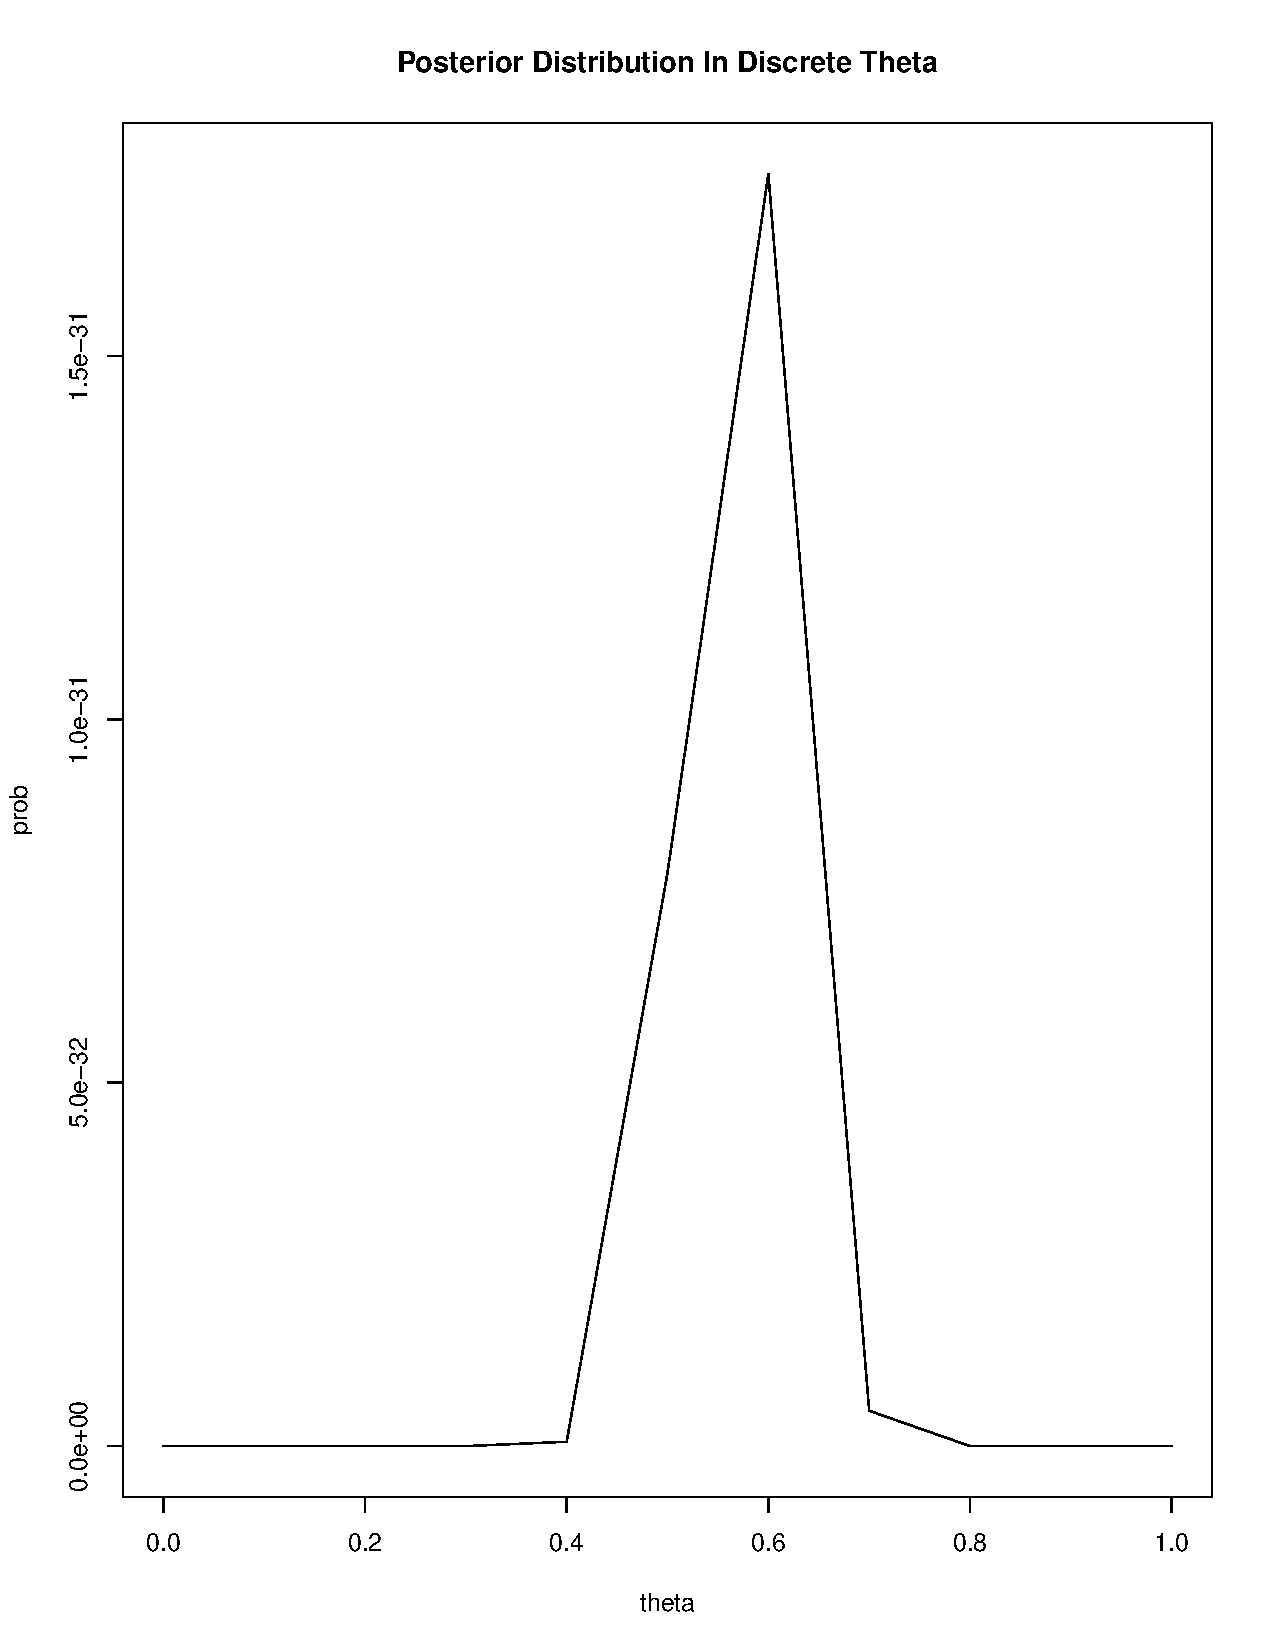
\includegraphics[width=75mm, scale=0.8]{5iiiplot.pdf}

\subsection{iv}
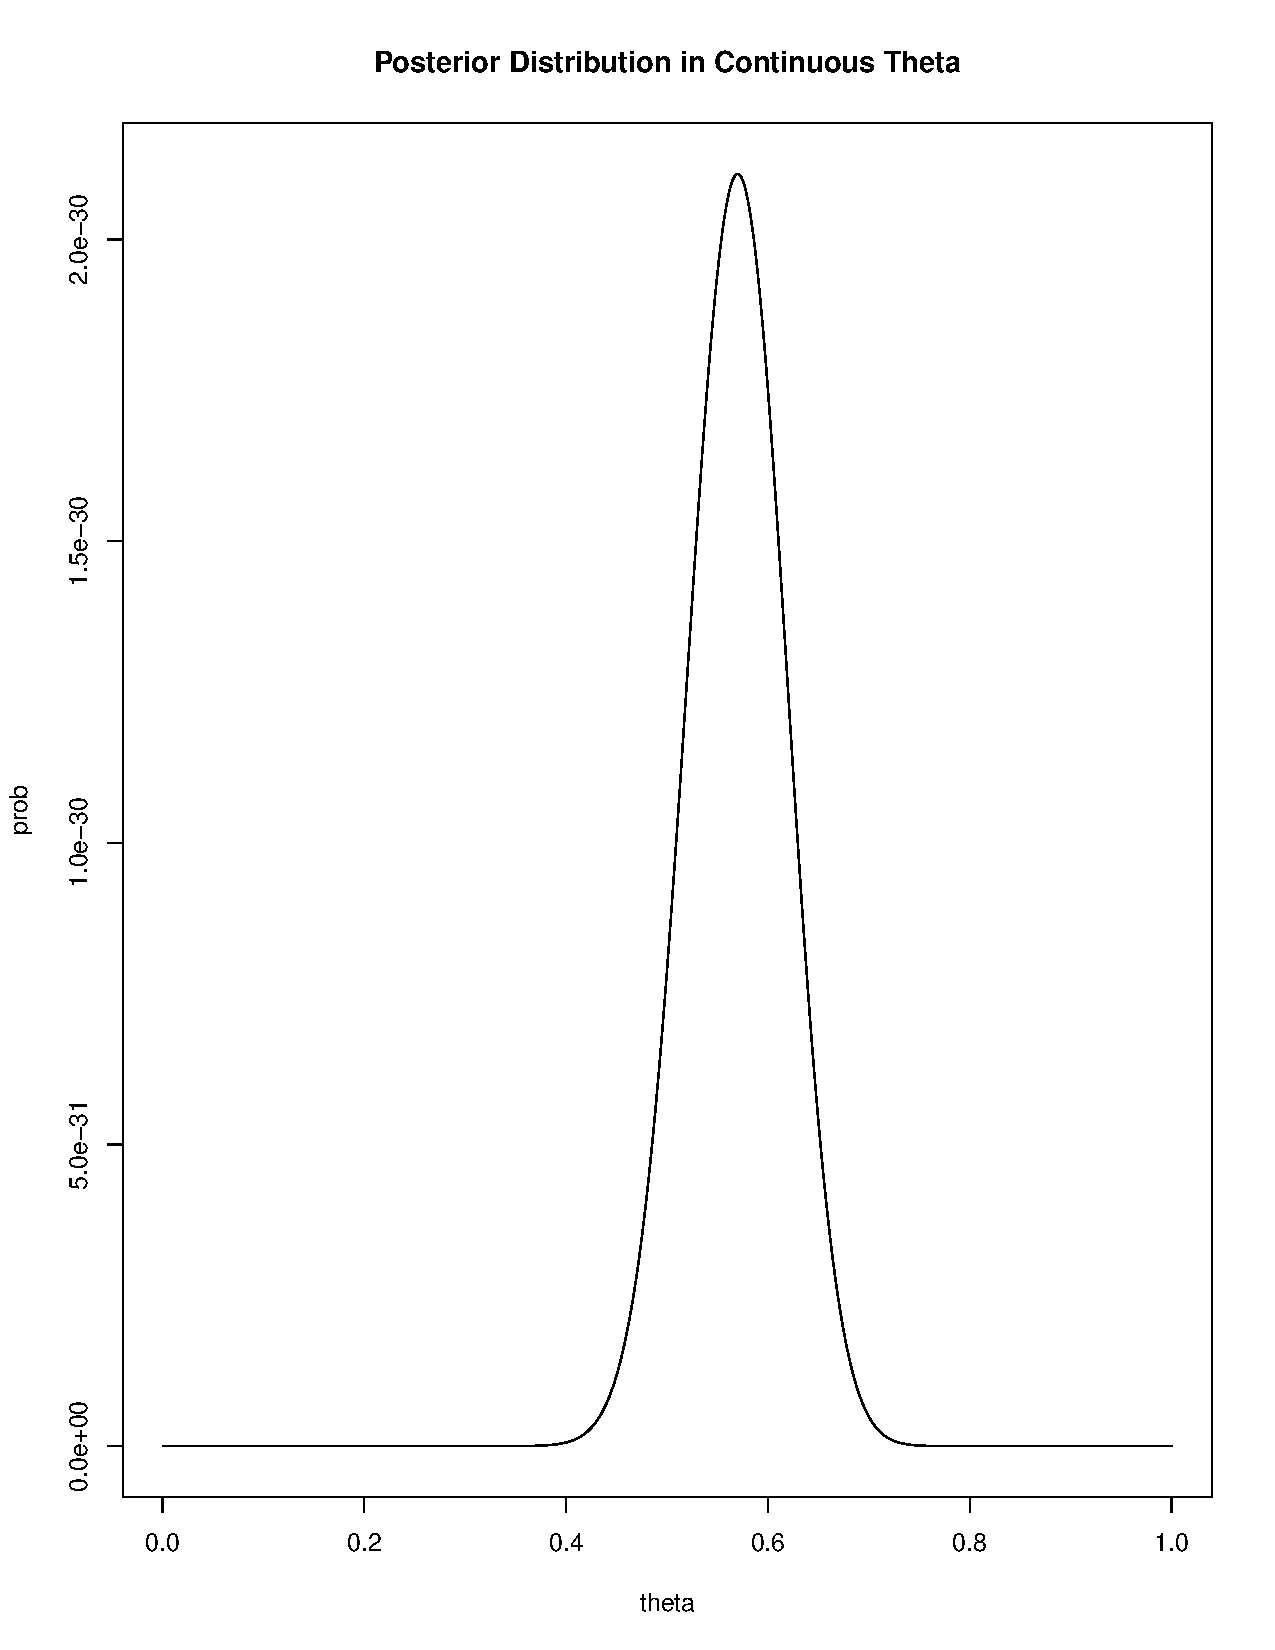
\includegraphics[width=75mm, scale=0.8]{5ivplot.pdf}

\subsection{v}
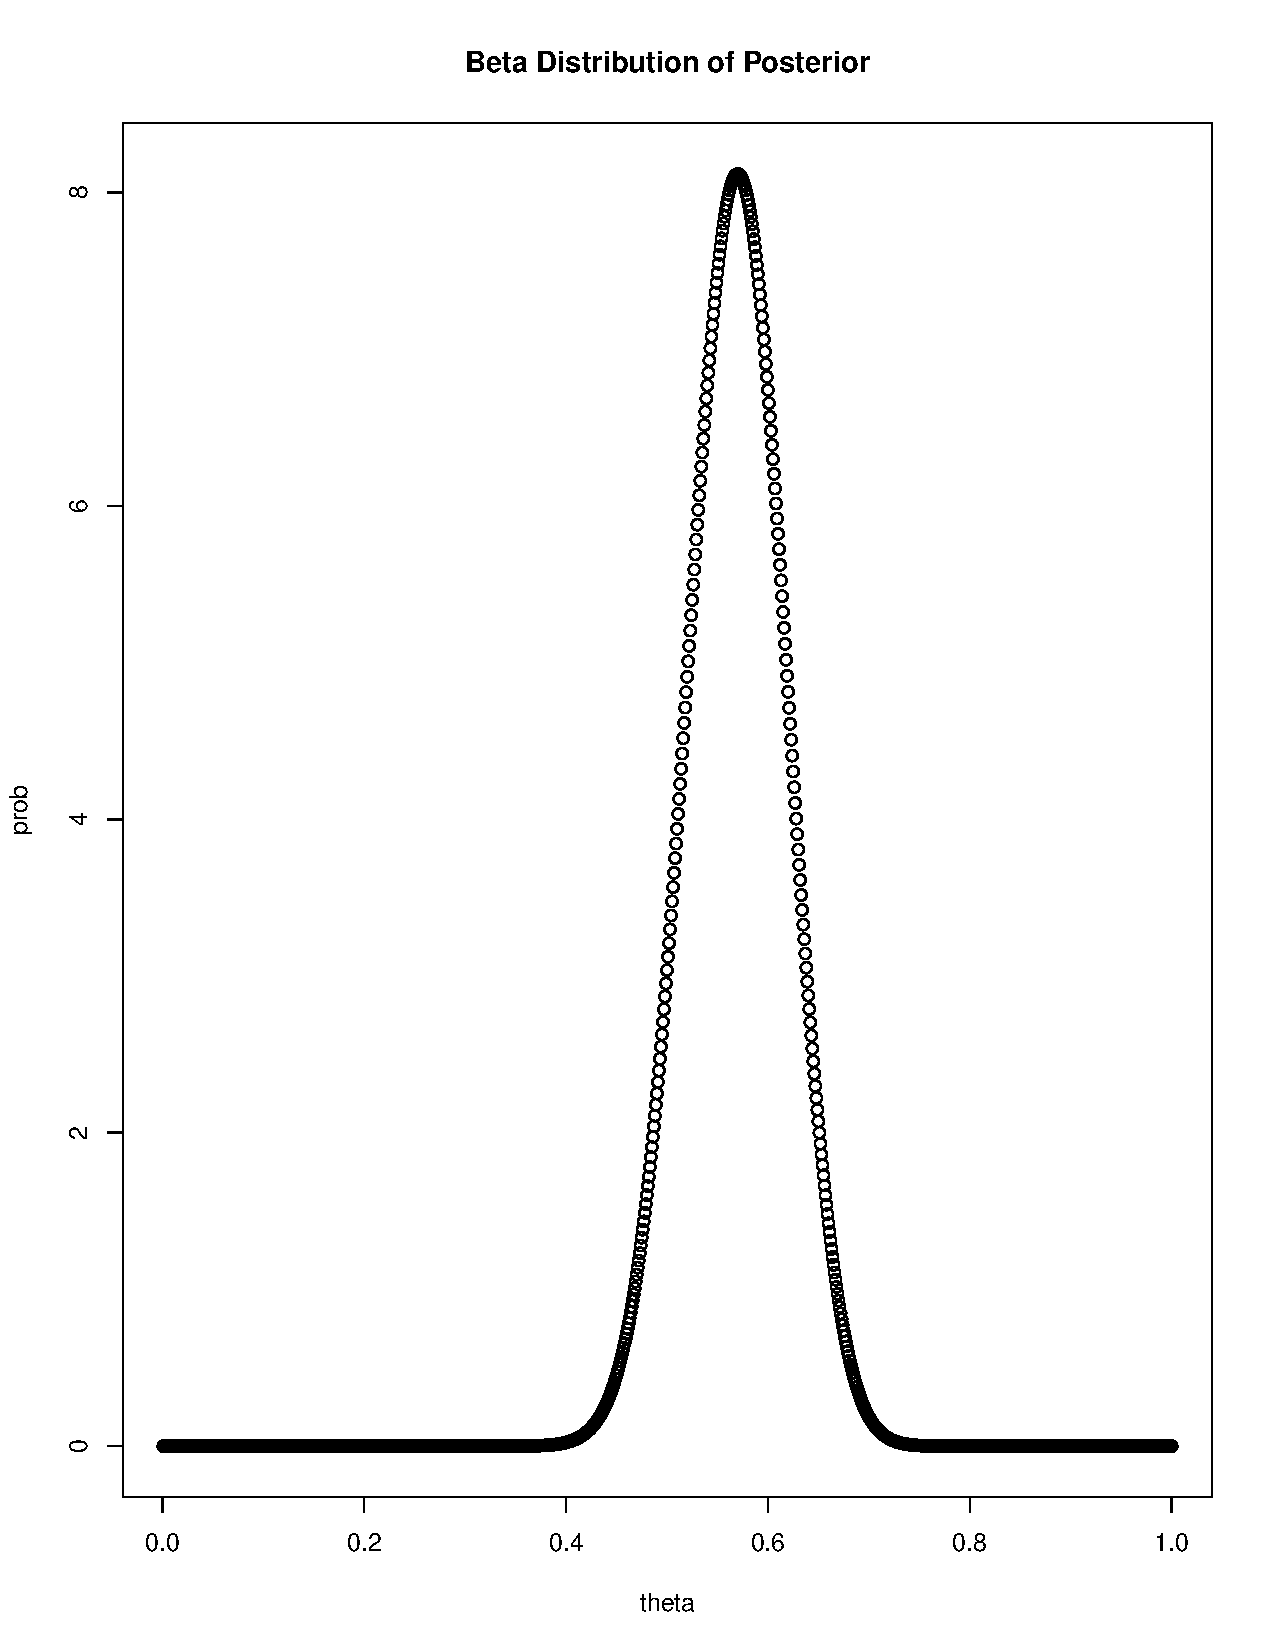
\includegraphics[width=75mm, scale=0.8]{5vplot.pdf}

The different plots show different variations of a "posterior distribution". In part ii), this shows a discretized plot of the likelihood function, whereas in part iii), there is now the introduction of a prior. IN part iv), this shows a more continuous versino of the posterior distribution. And then in v), this is the actual posterior distribution based on conjugate prior analysis.

\section{Problem 6}
We know that the beta priors for a binomial/bernoulli distribution is a conjugate prior. So the posterior distribution is of the form beta(A, B), where in this case, we solve and obtain: \\
$A = a+57$\\
$B = b+100-57$

The contour plots are shown here:

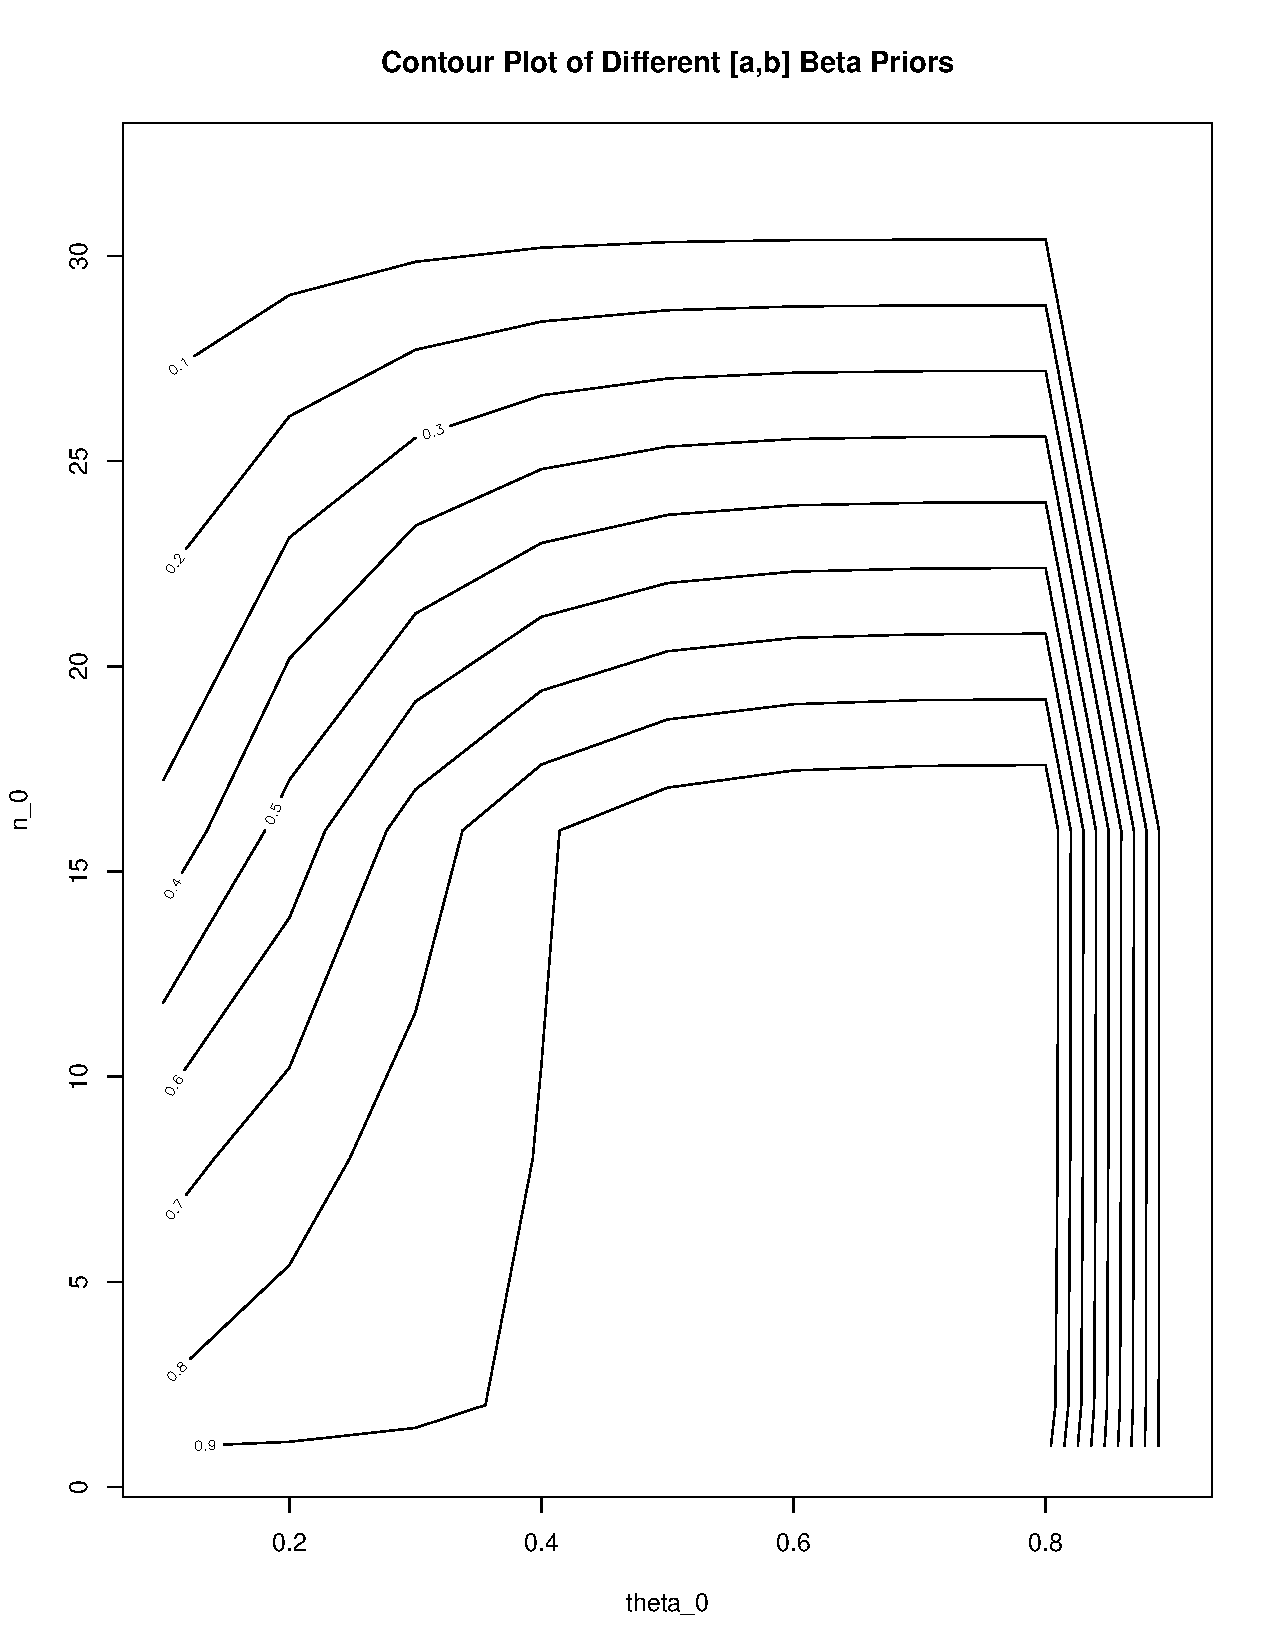
\includegraphics[width=75mm, scale=0.8]{6plot.pdf}

\end{document}
